\documentclass[12pt]{beamer}

\usepackage[utf8]{inputenc}
\usepackage{amsmath}
\usepackage{hyperref}
\usepackage{graphicx}
\usepackage{caption}
\usepackage{subcaption}
\usepackage[style=ext-authoryear, backend=biber]{biblatex}
\addbibresource{refs.bib}
\usepackage{csquotes}

\DeclareOuterCiteDelims{parencite}{\bibopenbracket}{\bibclosebracket}

\begin{document}

\begin{frame}{Learning invidivdual intrinsic rewards (LIIR) \parencite{learn_intr_rewards}}
  \begin{itemize}
    \item learn intrinsic reward per agent
    \begin{itemize}
      \item MLP ($\eta$) with 2 hidden layers~\parencite{intrinsic_reward}
      \item state and action as input
      \item[$\rightarrow$] to diversify
      \item[$\rightarrow$] to learn faster
    \end{itemize}
    \pause
    \item update $\theta$ with regards to proxy reward
    \item update $\eta$ with regards to extrinsic rewards via meta-gradient
  \end{itemize}
\end{frame}

\begin{frame}
  \begin{figure}
    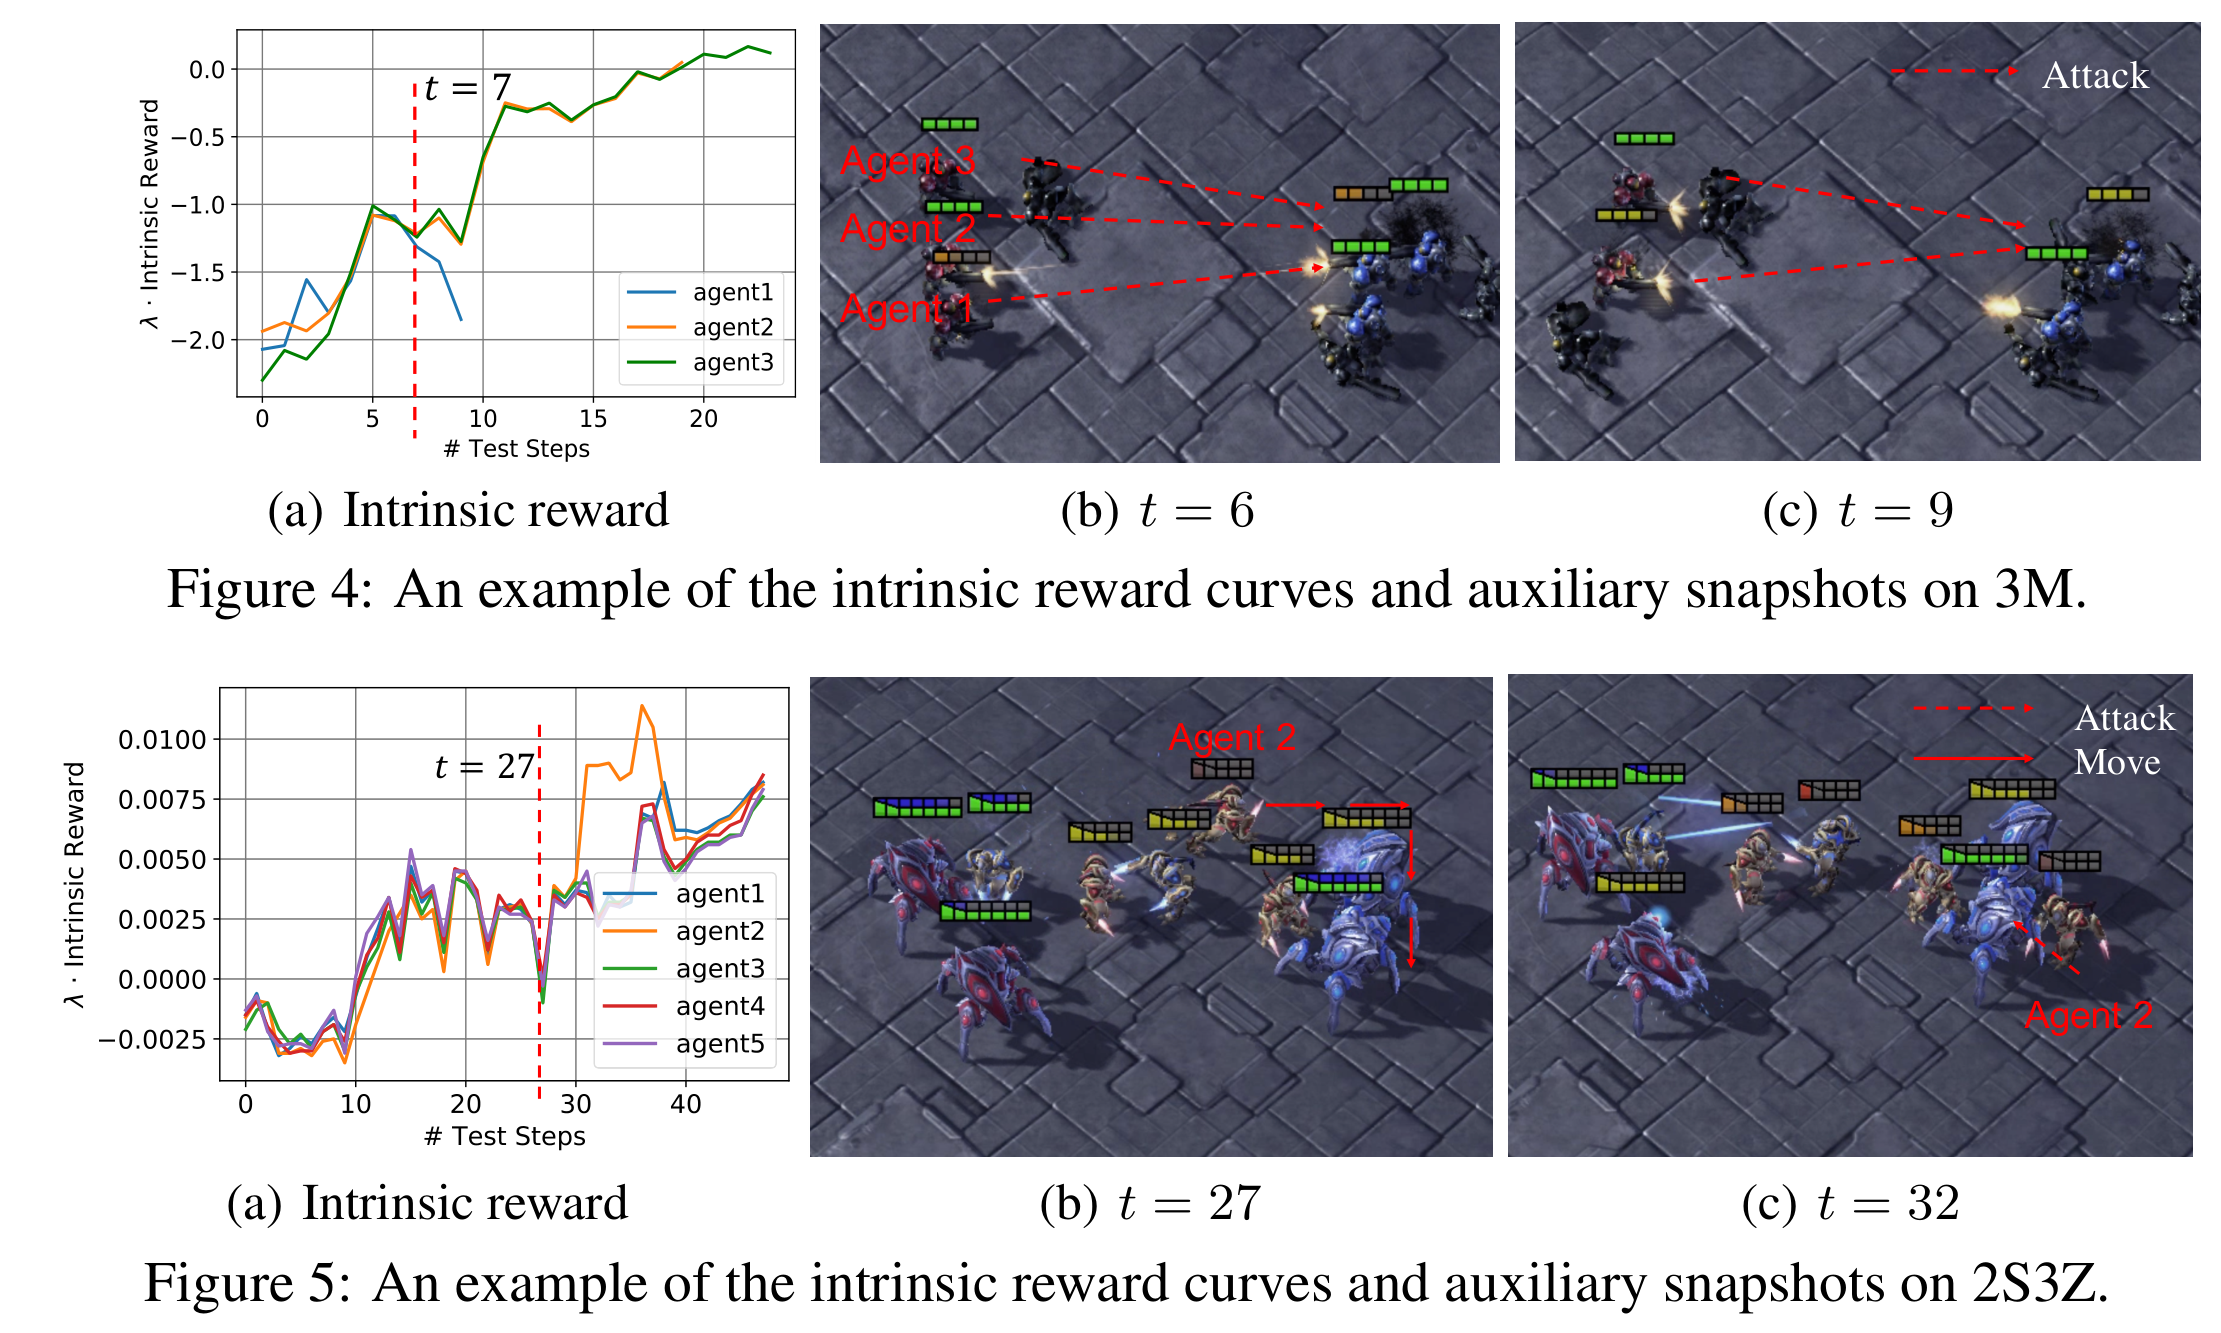
\includegraphics[width=\textwidth, height=\textheight, keepaspectratio]{./demonstration.png}
  \end{figure}
\end{frame}

\begin{frame}
  \begin{figure}
    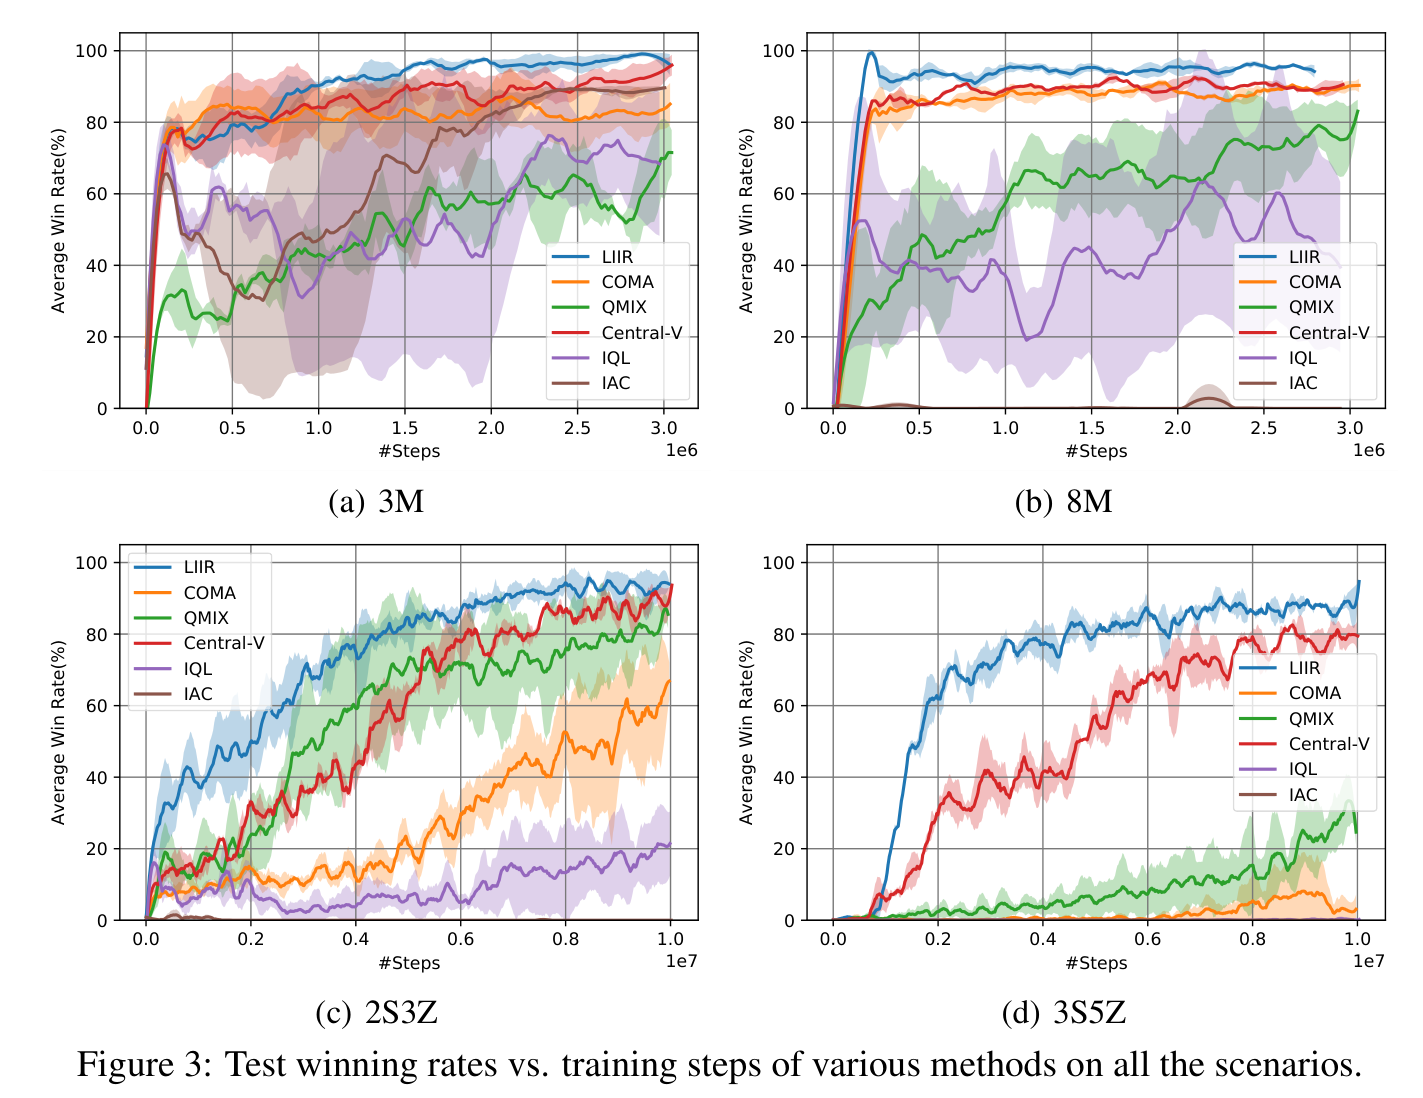
\includegraphics[width=\textwidth, height=\textheight, keepaspectratio]{./results.png}
  \end{figure}
\end{frame}

\end{document}
